% write cover letter this way

\documentclass{letter}

\usepackage{graphicx}

\usepackage[letterpaper, left=40mm, right=40mm, top=15mm]{geometry}

\signature{Huan Quang Bui}
\address{Huan Quang Bui \\ 8347 Mayflower Hill \\ Waterville, Maine}

\begin{document}
	\begin{letter}{Charles Conover \\Colby College\\William A. Rogers Professor of Physics\\ Department of Physics and Astronomy}
		\opening{Dear Professor Conover,}
		I am a rising sophomore at Colby College pursuing a double-major in Physics and Mathematical Sciences with a Concentration in Statistics. I am writing to express my interest in working in your lab this summer as a Student Research Assistant. Having realized the significance of studying and understanding Rydberg systems, I would welcome the opportunity to continue contributing to both ongoing and upcoming projects at your lab, namely precision measurements of Rydberg transitions in potassium and modifying the current apparatus to support higher experiment repetition rates and allow for atom-atom collision experiments.
		
		From PH241-242 and the chance to assist you in your lab since the beginning of JanPlan, I have learned many valuable skills necessary for experimental atomic laser spectroscopy. Based on a previously built circuit and the schematics you provided, I constructed a new laser frequency-locking electronics with variable time constants. In the lab, I learned the basic principles of laser locking, retuning and locking lasers when they come unlocked, and computer-based spectroscopy data acquisition using IGOR Pro. Given locked lasers and a millimeter-wave source that are set to drive a certain transition, I am capable of taking and analyzing absorption data for various field strengths through curve-fitting. I am comfortable with multiple operating systemss (MacOS, Windows, Linux) and experienced in coding in Java and Python. I am also currently learning \LaTeX{} in my leisure time through writing an introductory study guide for special relativity, based on the material from PH241. 
		
		Additionally, I have been substantially augmenting my understanding of the theoretical aspects of the experiment. This semester, I am taking PH242: Modern Physics II, PH311: Classical Mechanics, and MA253: Linear Algebra, which equip me with necessary tools to self-explore and study quantum mechanics, with Shankar's \textit{Principles of Quantum Mechanics} as my guiding text. I am also studying specific chapters from Berman and Malinovsky's \textit{Principles of Laser Spectroscopy and Quantum Optics} and reading papers on Rydberg systems and magneto-optical trapping to understand the experiment in more detail. 
	
		Thank you for your consideration. I feel very fortunate to have been working in your lab and feeling motivated to study physics beyond my curriculum. I look forward to the opportunity to continue assisting you this summer. 
		
		Yours sincerely,
		
		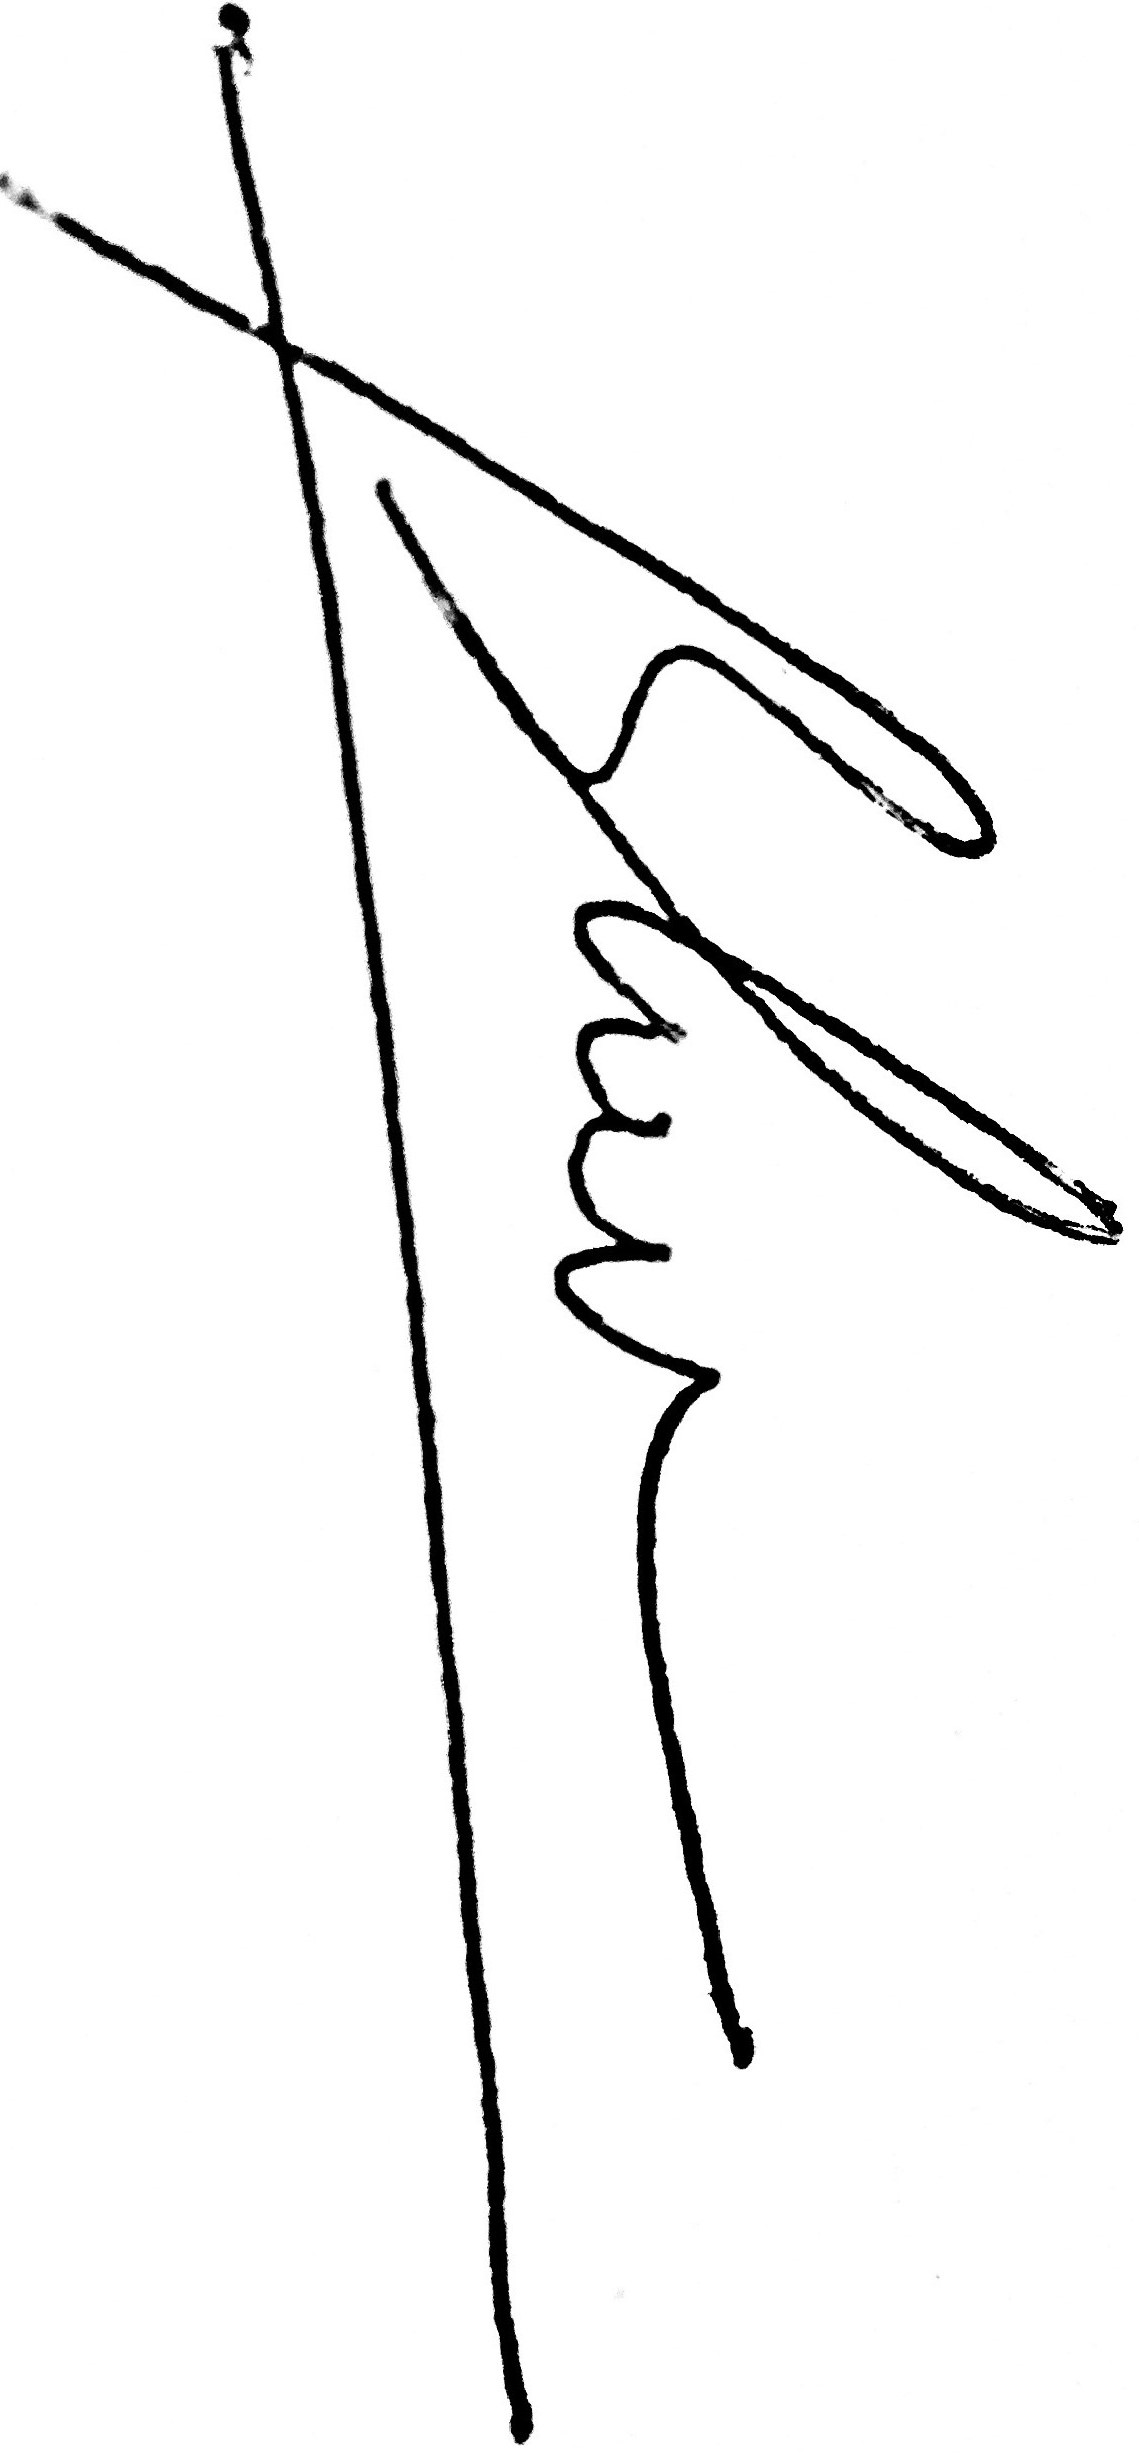
\includegraphics[scale=0.03, angle=90]{IMG_0789.JPG}
		
		Huan Quang Bui
		
	\end{letter}
	
\end{document}


